\documentclass[letterpaper,twocolumn]{article}

% Math packages
\usepackage{amsthm}
\usepackage{amsmath}
\usepackage{amssymb}

% For more complicated table formatting
\usepackage{multirow}
\usepackage{tabularx}
\newcolumntype{L}[1]{>{\raggedright\let\newline\\\arraybackslash\hspace{0pt}}m{#1}}
\newcolumntype{C}[1]{>{\centering\let\newline\\\arraybackslash\hspace{0pt}}m{#1}}
\newcolumntype{R}[1]{>{\raggedleft\let\newline\\\arraybackslash\hspace{0pt}}m{#1}}

% Remove line spaces between items of enumerate and itemize
\usepackage{enumitem}
\setlist{noitemsep}

% Adds double bracket symbols
\usepackage{stmaryrd}

% Allows to create negation symbols
\usepackage{MnSymbol}

% General math symbols
\DeclareMathOperator{\Id}{Id} % Identity function

% Theorem styles

%\renewcommand\thesubsection{\thesection.\Alph{subsection}}
%\renewcommand{\theequation}{\thechapter.\arabic{equation}}

\newtheorem{assump}{Assumption}
\renewcommand*{\theassump}{\Roman{assump}}

\newtheorem{axiom}[equation]{Axiom}
\newtheorem{defn}[equation]{Definition}
\newtheorem{prop}[equation]{Proposition}
\newtheorem{coro}[equation]{Corollary}
\newtheorem{thrm}[equation]{Theorem}

%\theoremstyle{definition}

\newenvironment{remark}{\emph{Remark}.}{}
\newenvironment{rationale}{\emph{Rationale}.}{\qed}
\newenvironment{justification}{\emph{Justification}.}{\qed}
\renewenvironment{proof}{\emph{Proof}.}{\qed}


% LOGIC symbols
% -------------

% Boolean symbols and algebra
\def\Bool{\mathbb{B}}
\def\TRUE{\textsc{true}}
\def\FALSE{\textsc{false}}
\def\AND{\wedge}
\def\bigAND{\bigwedge}
\def\OR{\vee}
\def\bigOR{\bigvee}
\def\NOT{\neg}

% Logical context and related symbols
\def\logCtx{\mathcal{S}}
\def\vstmtSet{\mathcal{S}_\textsf{v}}
\def\dstmtSet{\mathcal{S}_\textsf{d}}
\newcommand{\pAss}[1][\mathcal{S}] {\mathcal{A}_{#1}}
\DeclareMathOperator{\truth}{truth}

% Experimental test symbols
\newcommand{\exptSet}{\mathcal{E}}
\newcommand{\expt}[1][e] {\mathsf{#1}}
\DeclareMathOperator{\result}{result}
\def\SUCCESS{\textsc{success}}
\def\FAILURE{\textsc{failure}}
\def\UNDEF{\textsc{undefined}}

% Statements
\def\tautology{\top} % Tautology
\def\contradiction{\bot} % Contradiction
\newcommand{\stmt}[1][s] {\mathsf{#1}} % Statement
\newcommand{\tstmt}[1][s] {\bar{\mathsf{#1}}} % Theoretical statement

% Relationships between statements
\def\comp{\doublefrown} % Compatibility
\def\ncomp{\ndoublefrown} 
\def\narrower{\preccurlyeq} % Narrowness
\def\nnarrower{\npreccurlyeq}
\def\snarrower{\prec}
\def\nsnarrower{\nprec}
\def\broader{\succcurlyeq} % Broadness
\def\nbroader{\nsucccurlyeq}
\def\sbroader{\succ}
\def\nsbroader{\nsucc}
\def\indep{\upmodels} % Independent
\def\nindep{\nupmodels}

% Experimental domains and related symbols
\newcommand{\edomain}[1][D] {\mathcal{#1}} % Experimental domain
\newcommand{\tdomain}[1][D] {\bar{\mathcal{#1}}} % Theoretical domain
\newcommand{\basis}[1][B] {\mathcal{#1}} % Basis
\newcommand{\resPoss}[1][x] {\mathring{#1}} % Residual possibility
\newcommand{\estPoss}[1][x] {\dot{#1}} % Established possibility

% Formatting for experimental relationships
\newcommand{\erel}[1][r] {#1}

% Formatting for sentence statements
\newcommand{\statement}[1] {\emph{``#1"}}

% Formatting for reference
\newcommand{\refStmt}[1][r]{\textbf{#1}}

\DeclareMathOperator{\ver}{ver}
\DeclareMathOperator{\fal}{fal}
\DeclareMathOperator{\und}{und}

\DeclareMathOperator{\interior}{int}
\DeclareMathOperator{\exterior}{ext}

% Level of detail
\def\eqgran{\doteq}
\def\finer{\leqdot}
\def\nfiner{\nleqdot}
\def\coarser{\geqdot}
\def\sfiner{\lessdot}
\def\scoarser{\gtrdot}

\usepackage{graphicx}
\usepackage{hyperref}
\hypersetup{
	colorlinks=true,
	citecolor=blue,
	urlcolor=blue,
	linkcolor=blue
}
\urlstyle{same}
\usepackage[font=scriptsize]{caption}

\begin{document}

\title{Counting evolutions: a simple foundation for thermodynamics}
\author{Gabriele Carcassi\footnote{carcassi@umich.edu}, Christine A. Aidala, et al \\ University of Michigan}

\date{\today}

\maketitle

\begin{abstract}
	In this work we present the core ideas at the heart of a new approach to the foundations of thermodynamics. The premise is to focus on the count of evolutions: the possible ways the state of a system can evolve in time. We see that in a deterministic process the evolutions can never diverge and in a reversible one they can never merge. This means that the count of evolutions per state can never decrease under a deterministic process and it is maximized at equilibrium. We show how this simple idea can be used as a straightforward foundation for thermodynamics and how it relates to other notions of entropy in physics.
	
	This work is part of Assumptions of Physics, a project that aims to identify a handful of physical principles from which the basic laws can be rigorously derived  (\url{https://assumptionsofphysics.org}).
\end{abstract}


\section{Introduction}

This working draft summarizes the status of our work on a new approach to the foundations of thermodynamics and is intended to gather early feedback. Rather then derive thermodynamics bottom-up from a particular microscopic model, we want to derive it top-down from a set of requirements on the dynamics of the system. The results we find are, then, independent of the microscopic dynamics in the sense that they can in principle be realized in different ways. This is both more in line with the aims of the founders of thermodynamics and justifies why thermodynamic concepts have been successful in fields beyond physics. Moreover, in our approach thermodynamics is found as a specialization of a more general model, which we believe can be used as a common foundation for the different types of mechanics.

In a nutshell, we characterize processes in general terms, as the description of all possible ways that the system can evolve in time, its possible evolutions, under a particular set of circumstances, as one can see in figures \ref{fig_single_evolution} through \ref{fig_with_equilibria}. Counting the possible evolutions plays a fundamental role, in much the same way that counting states plays a role in statistical mechanics. In a deterministic and reversible process, there is a one-to-one correspondence between initial and final states: the evolutions cannot merge or diverge. If the process is deterministic but not reversible, however, the same final state will be reached from different initial states, and the evolutions will merge. If the deterministic process reaches an equilibrium, there will be no more merging. We define process entropy to be the logarithm of the count of evolutions per state, which we find to have the basic properties we associate with entropy: it is linear under system composition of independent systems, can never decrease under a deterministic process, increases if the process is non-reversible and is maximized at equilibrium. This gives us a conceptually crisp physically meaningful concept that is tied to irreversibility and equilibria in a very natural way.

There are many technical details that are required to make the above characterization formally rigorous, mostly due to the proper handling of infinities. However, those do not really change the overall intuition, which we believe is the main strength of the approach. Therefore, in this paper, we will only give a conceptual overview leaving the formal details to other papers. This will leave the key physical insight more directly accessible, and also result in a narrative that can be used directly in an introductory course of thermodynamics.

The paper is organized in three sections. In the first we will present a simple framework to characterize processes in general terms. In the following section we will add the definitions and assumptions that are specific to thermodynamic processes and rederive the basic laws. In the last section we see how the concepts presented relate to the different branches of mechanics.

\section{States, processes and evolutions}\label{sec_process_entropy}

Our first task is to characterize processes in the most general terms. We assume we have a system and we want to study its behavior in a given set of circumstances. If the state space $X$ of the system represents all possible configurations the system can be found in, ultimately we want to characterize how the state changes in time. As depicted in figure \ref{fig_single_evolution}, we have a copy of the state space at each moment in time, and we call an \textbf{evolution} a trajectory $\lambda : T \to X$ that for each moment in time returns the state of the system. 

\begin{figure}[h]
	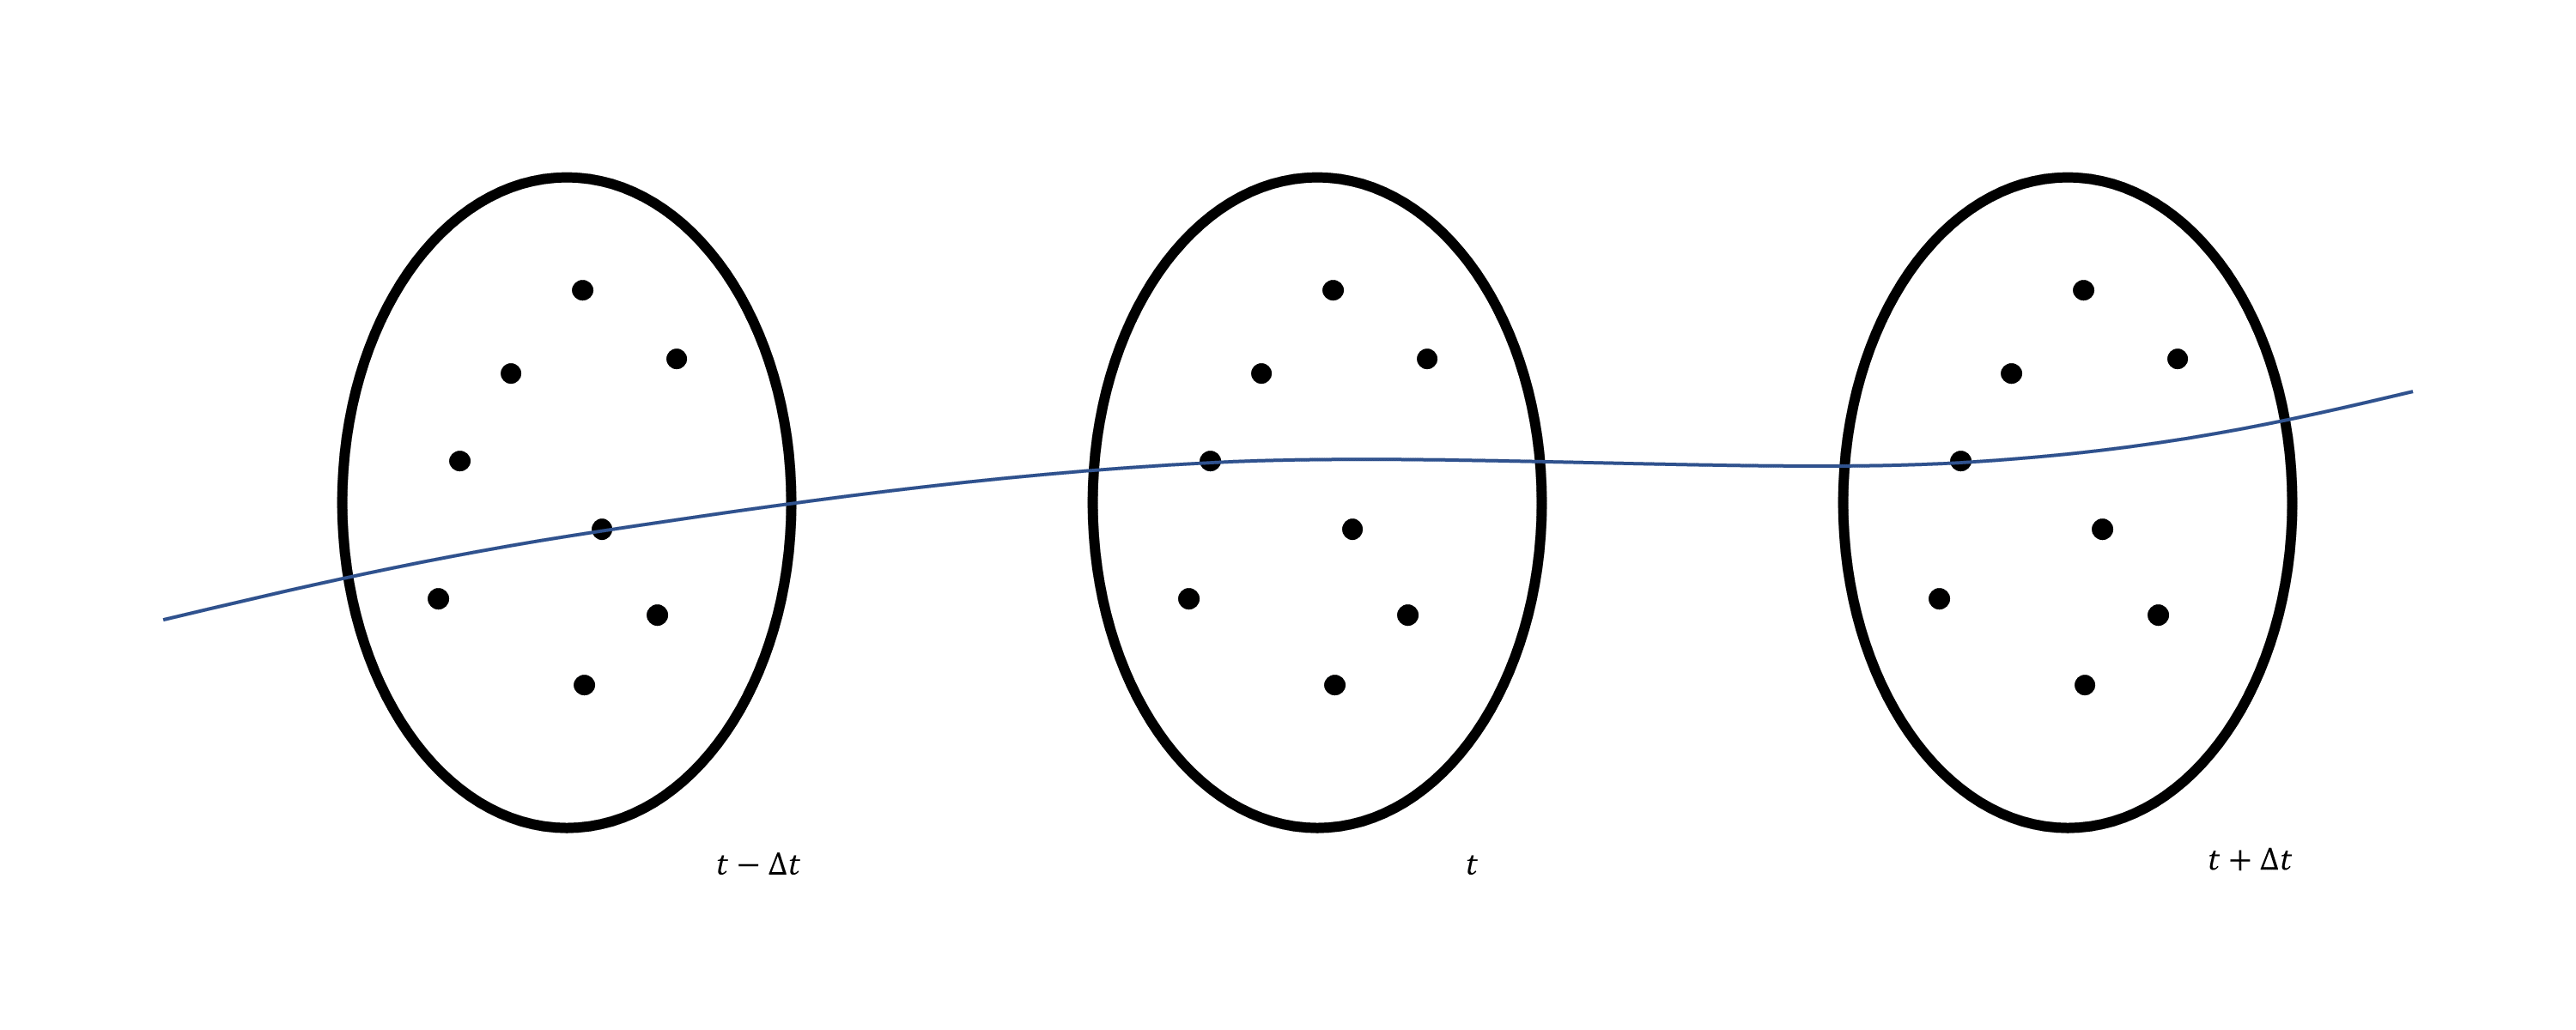
\includegraphics[width=\columnwidth]{images/Slide1.png}
	\caption{The three sets represent the state space of the same system at three different moments in time. The blue line is an evolution, which tells us the state of the system at all times.}\label{fig_single_evolution}
\end{figure}

Since not all evolutions will be allowed under all conditions, we characterize a \textbf{process} as the set of possible evolutions $E$, as we can see in figure \ref{fig_process}. Namely, a process tells us what can and cannot happen to a system in a given set of circumstances.\footnote{For example, a damped harmonic oscillator will allow trajectories whose oscillations degrade over time in a specific fashion.} We also assume we have a measure $\mu$ that allows us to determine the size of a set of evolutions, to ``count'' evolutions.\footnote{The full mathematical characterization is more complex: it will be a preorder that induces a family of measures, as to properly address sets of infinite relative sizes. However, these details do not change the overall intuition and would only distract from the key insights.} Note that a state $x_t$ at a particular time identifies a set of compatible evolutions $A(x_t) = \{ \lambda \in E \, | \, \lambda(t) = x_t \}$, those that pass through that state at that time. Using $\mu$ we can give a size to that set, which we can write as $\mu(A(x_t))$ or $\mu(x_t)$ for short.

\begin{figure}[h]
	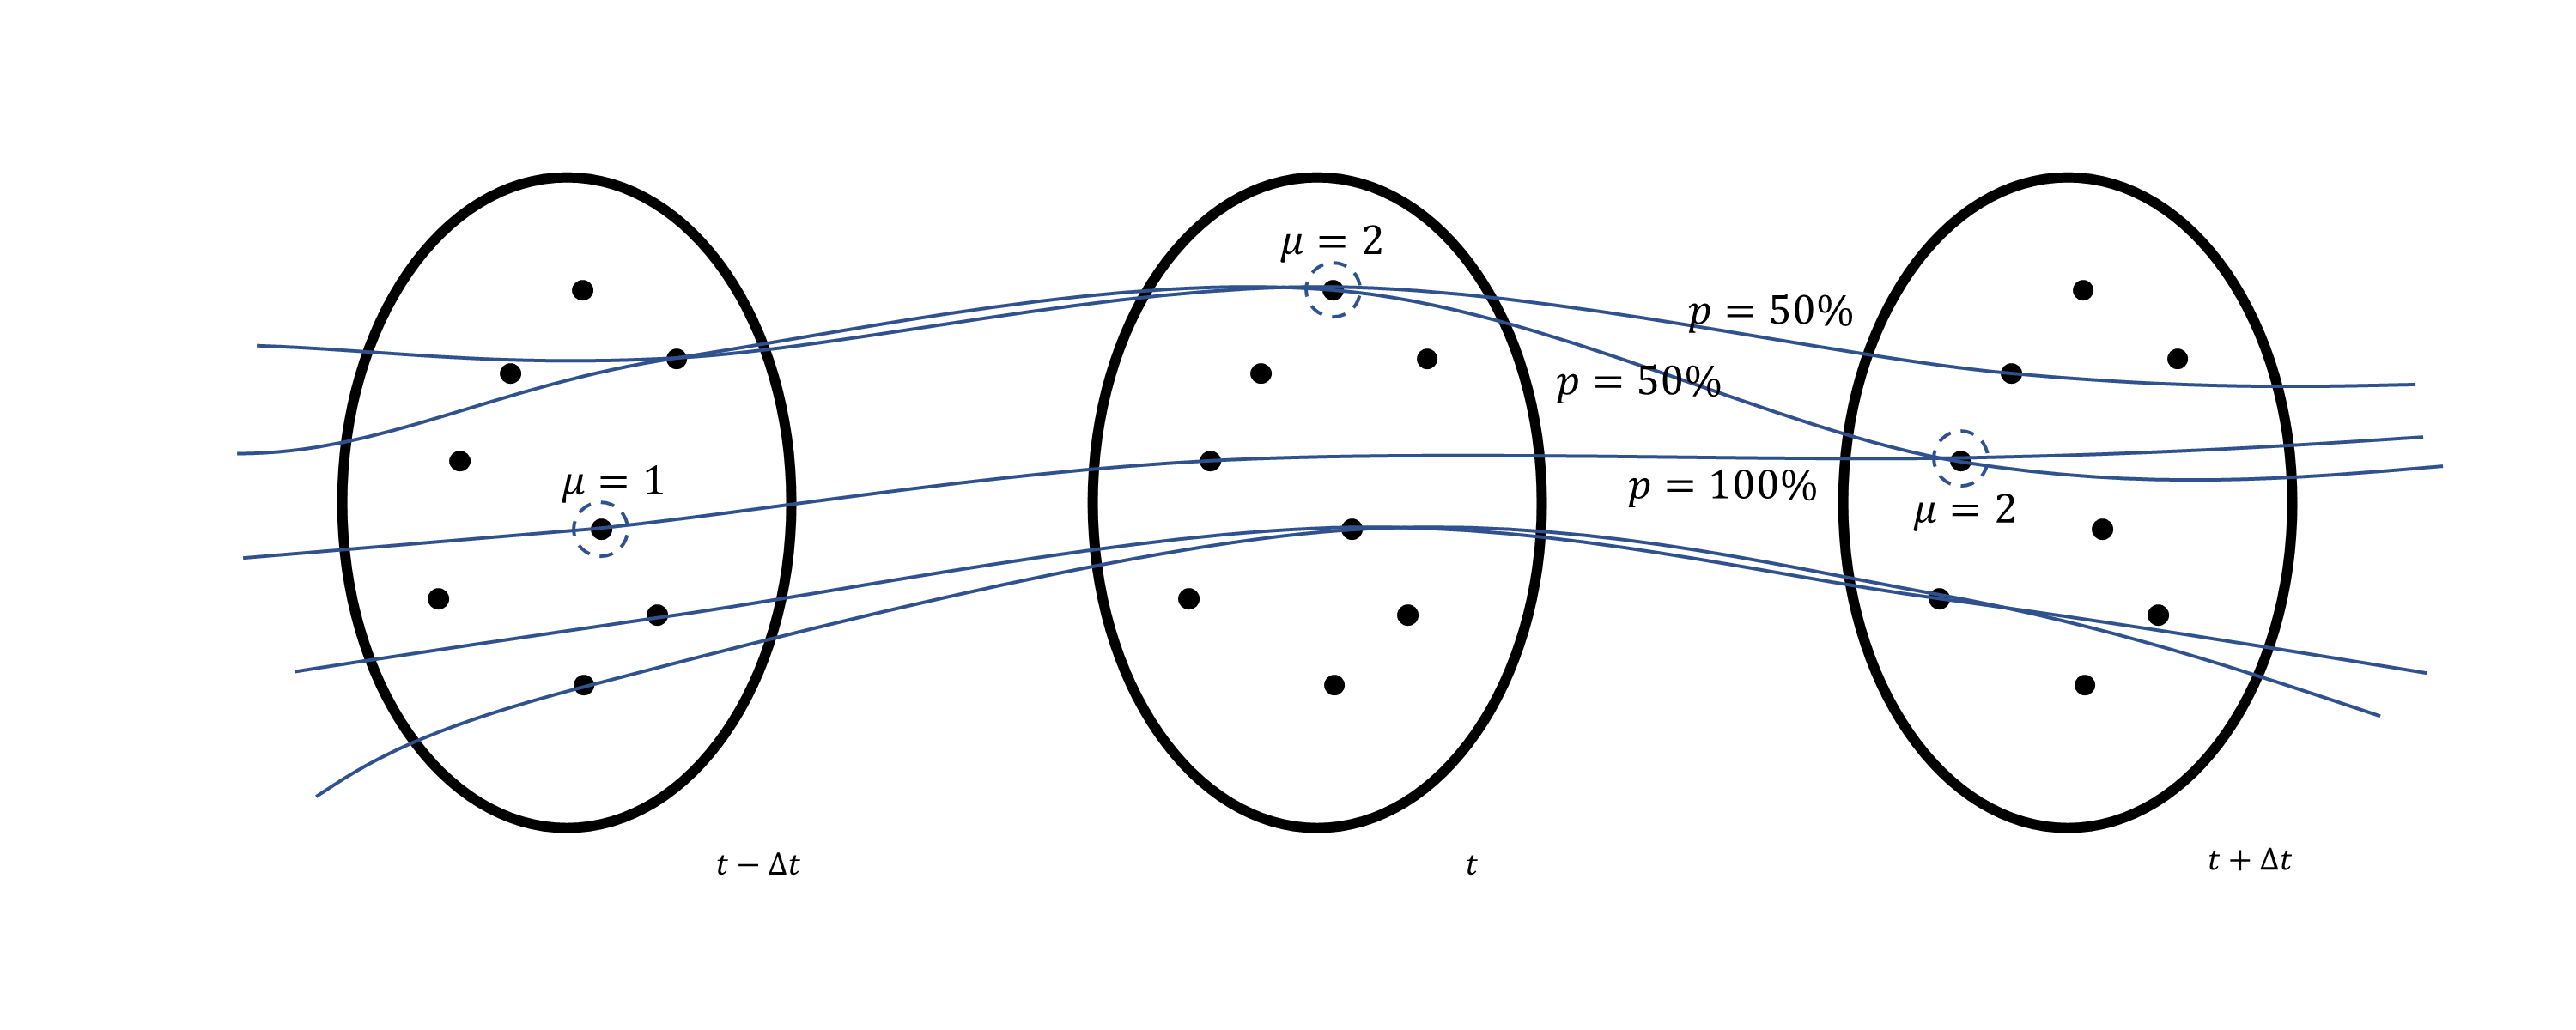
\includegraphics[width=\columnwidth]{images/Slide2.png}
	\caption{A process is characterized by the set of all possible evolutions. The measure $\mu$ allows us to express the size of a set of evolutions. The probability of transitioning from one state to another corresponds to the fraction of evolutions that starts in the first and also ends in the second.}\label{fig_process}
\end{figure}

Note that the probability of transitioning from one state to another during a process is linked to the possible evolutions and their count. In fact, calculating the probability of finding the state $x_{t+\Delta t}$ at $t+\Delta t$ given $x_t$ at $t$ means determining the fraction of evolutions that pass through $x_t$ that also pass through $x_{t+\Delta t}$. That is:
\begin{equation}
	P(x_{t+\Delta t} | x_t) = \frac{\mu(A(x_t) \cap A(x_{t+\Delta t}))}{\mu(A(x_t))}.
\end{equation}
Conceptually, the ability to count evolutions is equivalent to knowing all possible transition probabilities.\footnote{Technically, a single probability measure is not enough to define all these transitions at all scales, but the overall intuition remains.}

This very minimal characterization is enough for some basic definitions. We say a process is \textbf{deterministic} if the state at one time is enough to determine the state at all future times. We can see an example of such a process in figure \ref{fig_determinism}. In this case, if two different evolutions happen to reach the same state at a given time, they will also share all future states: evolutions can merge but cannot diverge. The count of evolutions per state over time can never decrease: $
\mu(\lambda(t)) \leq \mu(\lambda(t + \Delta t))$.

Deterministic processes can be characterized by a law of evolution. That is, we can write $\lambda(t+\Delta t) = f(\lambda(t), t)$ given a suitable function $f$ which may, in general, be time dependent. We can do this because, if we fix $x_t$, $P(x_{t+\Delta t} | x_t) = 1$ for one and only one future state and the law of evolution identifies that state. Insofar we are interested in making predictions, we are implicitly restricting ourselves to deterministic processes.

\begin{figure}[h!]
	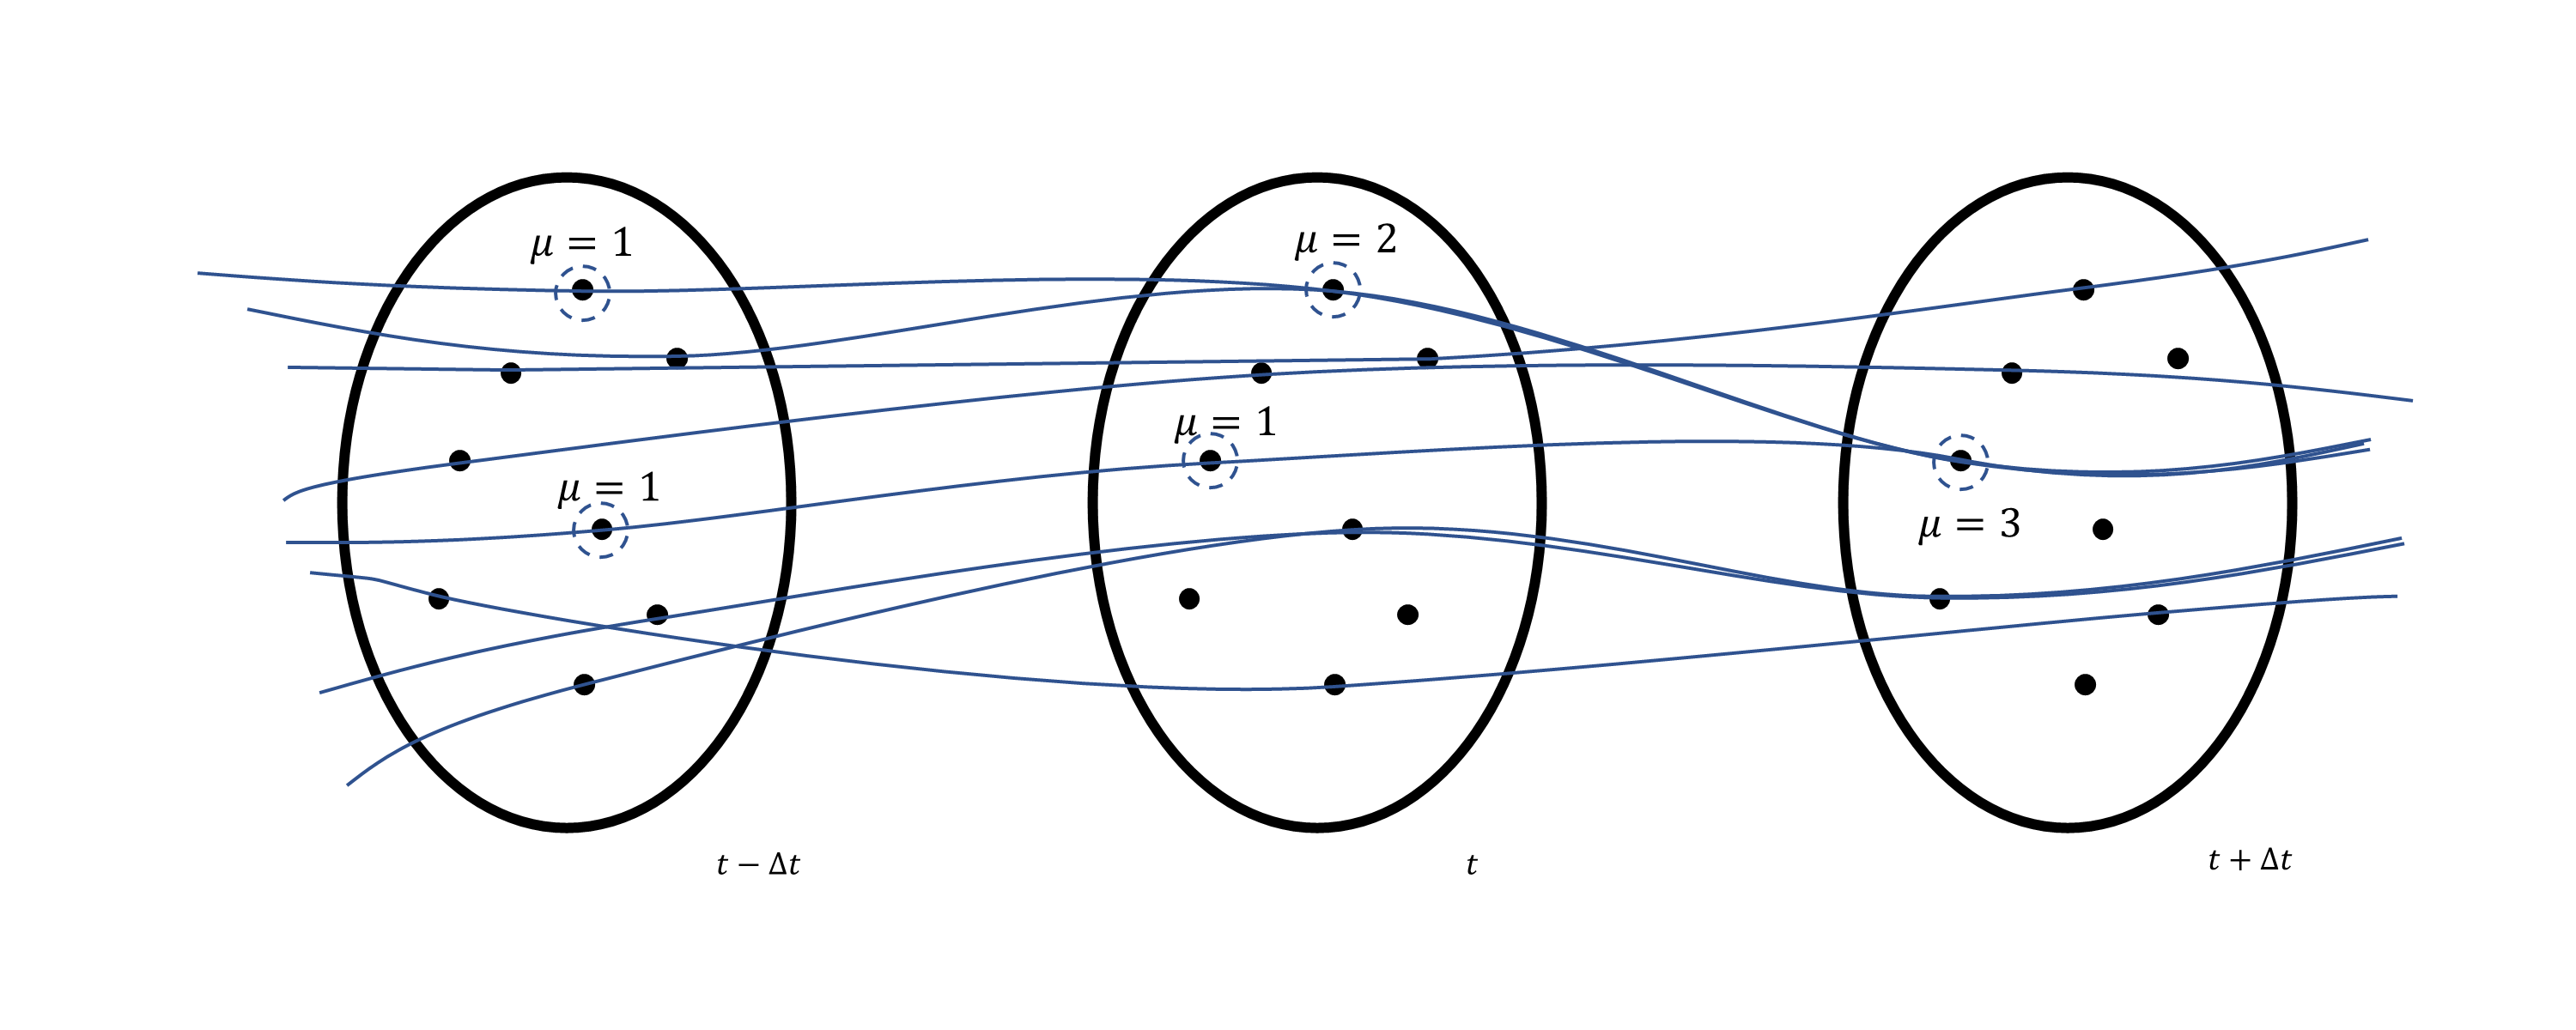
\includegraphics[width=\columnwidth]{images/Slide3.png}
	\caption{Deterministic process: the state at one time determines the state at future times. Evolutions can merge but not diverge in time. The number of evolutions per state cannot decrease.}\label{fig_determinism}
\end{figure}

Conversely, we say a process is \textbf{reversible} if the state at one time is enough to reconstruct the state at all past times.\footnote{Note that in some literature the ability to reconstruct the past is called retrodictability and does not coincide with thermodynamic reversibility (the ability to undo a change). This distinction appears in the context of continuous quantities and it is one of those technical considerations we will address in a more technical work. Our definition does recover thermodynamic reversibility, without having to assume the existence of a reverse process or a symmetry under time-reversal.} We can see an example of such a process in figure \ref{fig_reversibility}. In this case, if two different evolutions happen to reach the same state at a given time, they will also share all past states: evolutions can diverge but cannot merge. The count of evolutions per state over time can never increase: $
\mu(\lambda(t)) \geq \mu(\lambda(t + \Delta t))$.

\begin{figure}[h!]
	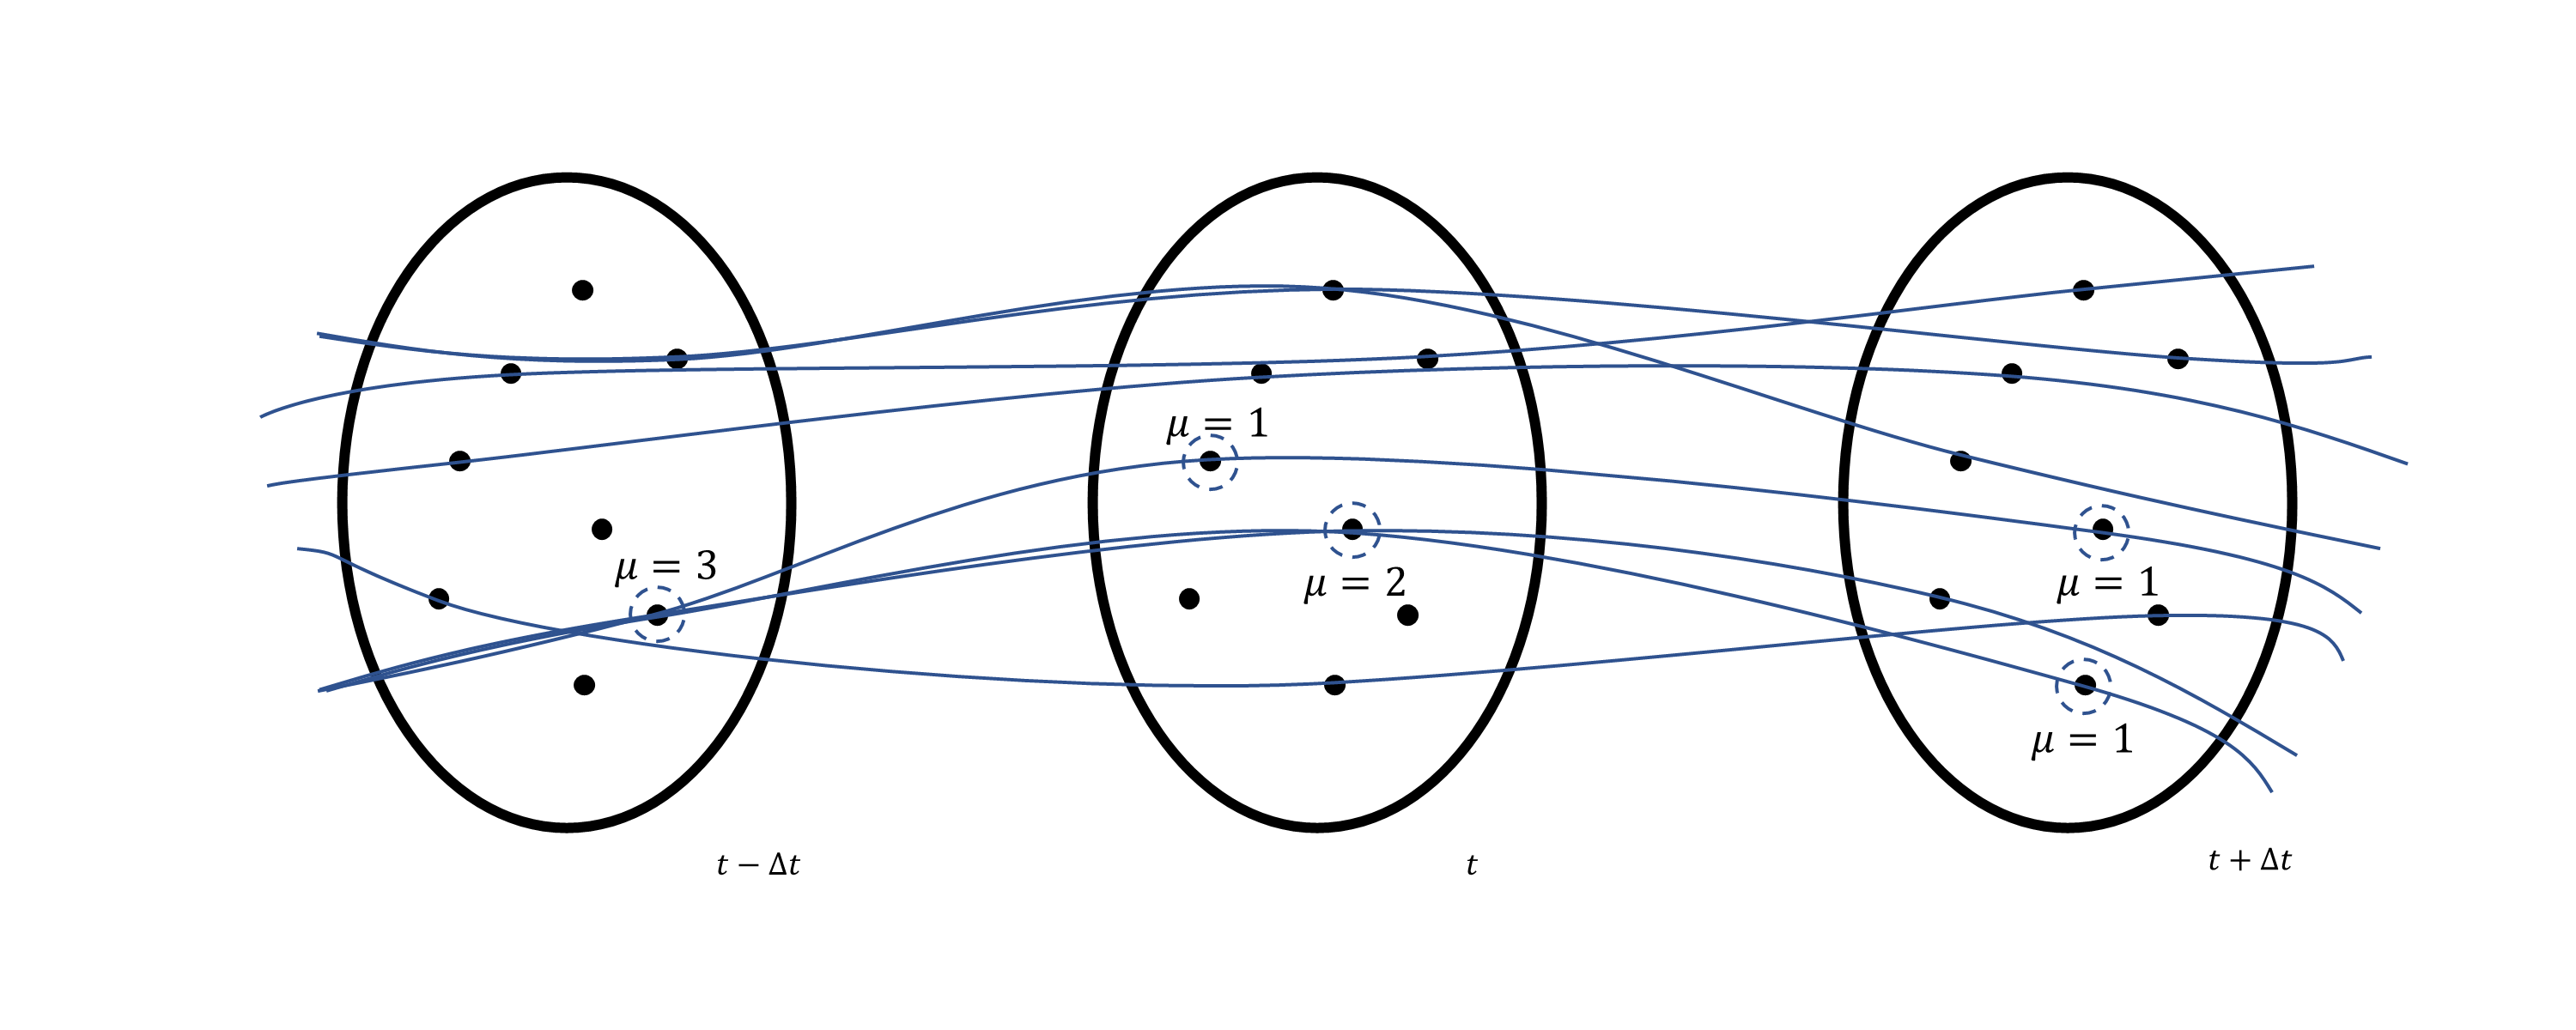
\includegraphics[width=\columnwidth]{images/Slide4.png}
	\caption{Reversible process: the state one time allows one to reconstruct the state at past times. Evolutions can diverge but not merge in time. The number of evolutions per state cannot increase.}\label{fig_reversibility}
\end{figure}



A process that is both deterministic and reversible, like the one in figure \ref{fig_detrev}, will never contain evolutions that split or merge. The count of evolutions per state over time will be a constant: $\mu(\lambda(t)) = \mu(\lambda(t + \Delta t))$.

\begin{figure}[h!]
	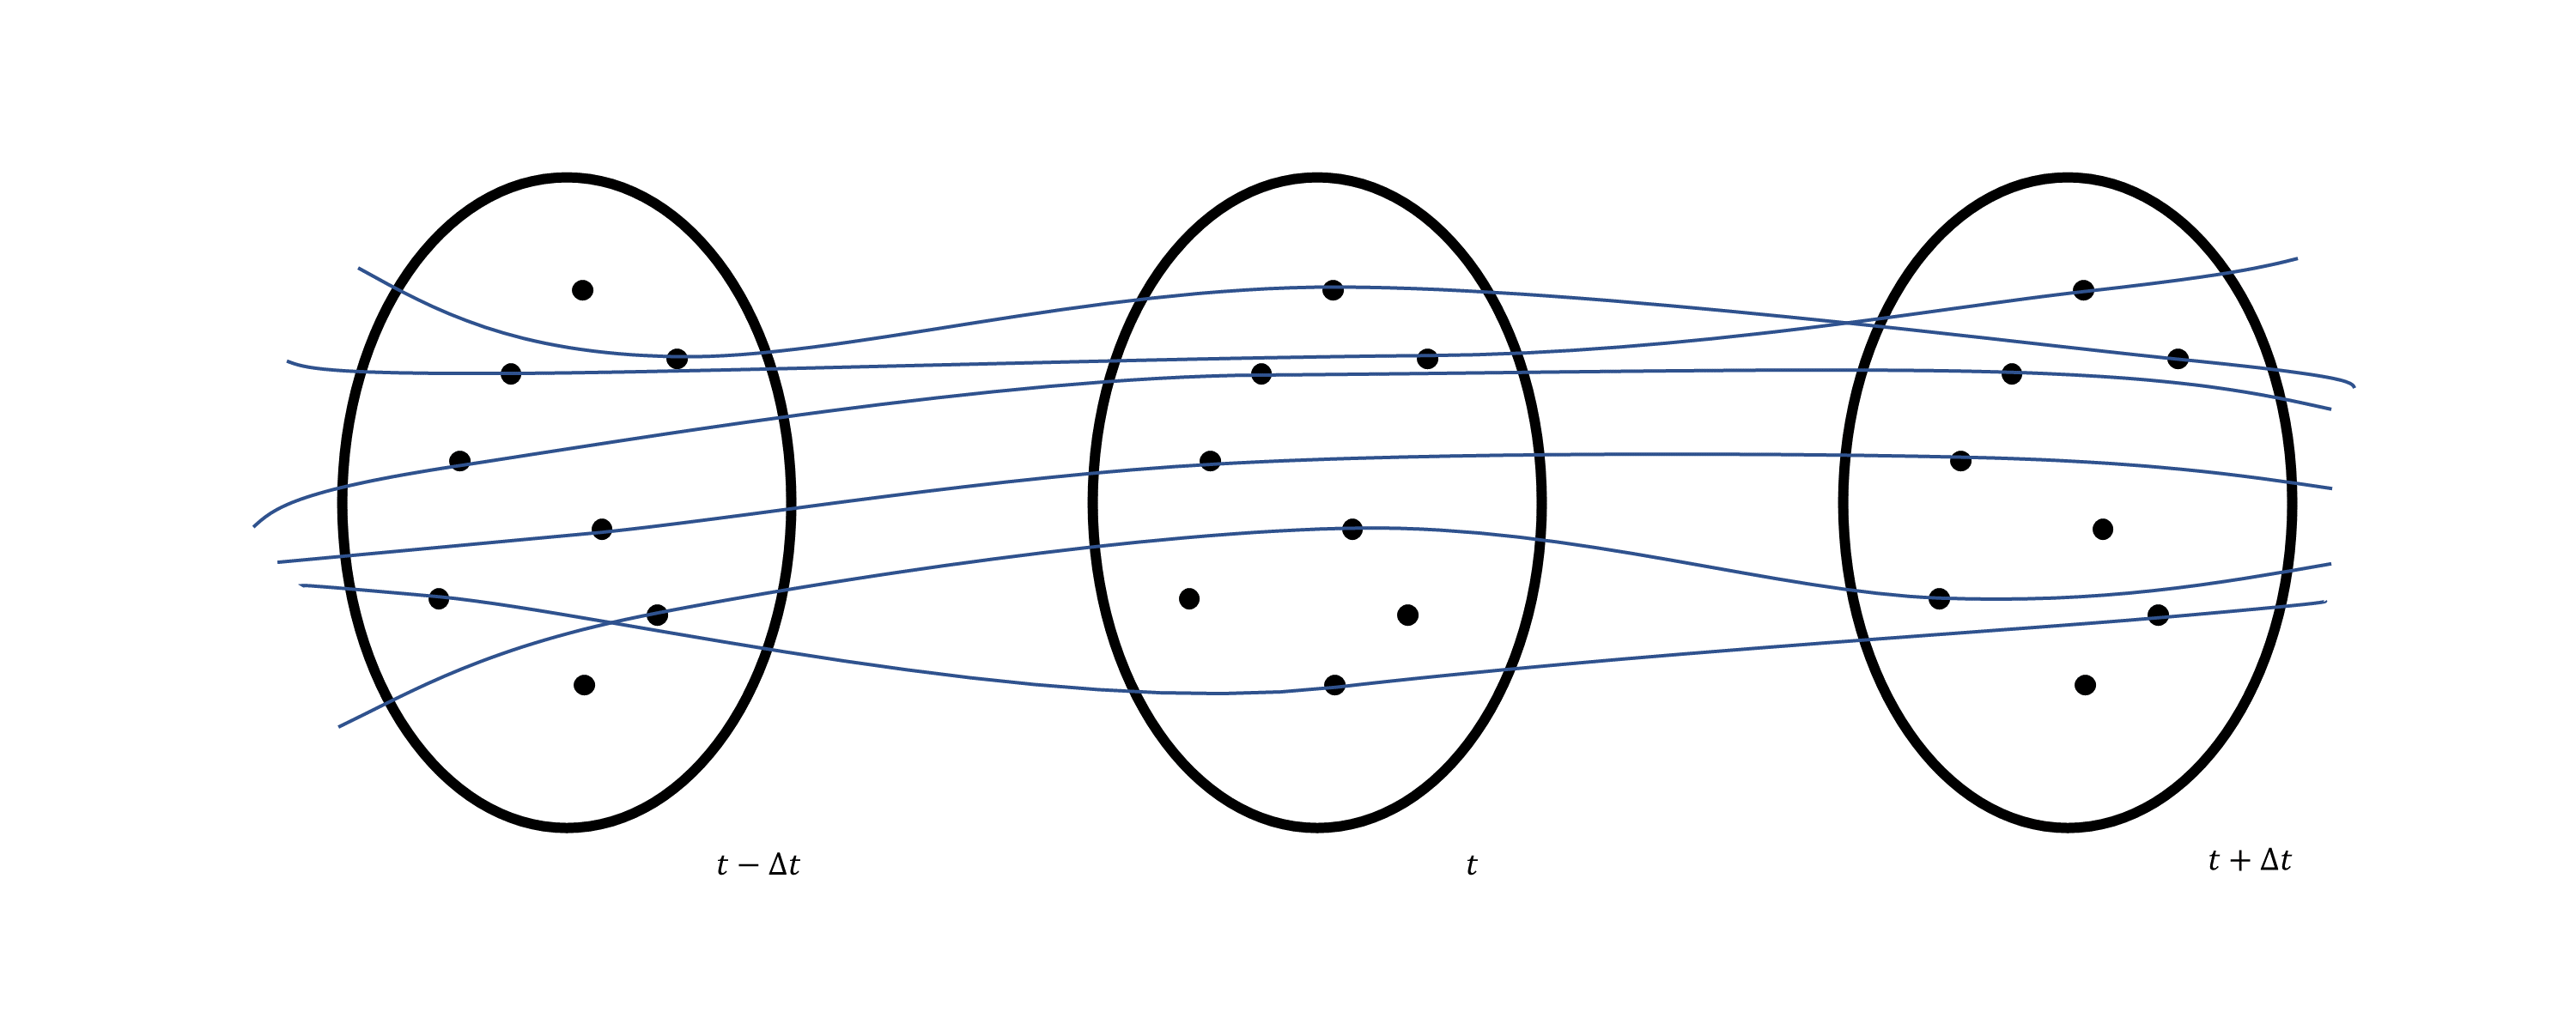
\includegraphics[width=\columnwidth]{images/Slide5.png}
	\caption{Determinism and reversibility. Evolutions cannot merge nor split. The number of evolutions per state cannot increase.} \label{fig_detrev}
\end{figure}


To finish, consider a \textbf{deterministic processes with equilibria}, like the one in figure \ref{fig_with_equilibria}. An equilibrium for a process is a state that, once it is reached, it is never left.\footnote{This characterization of equilibrium, though amply used in thermodynamic literature, is simplistic and technically does not quite work. However, it will suffice for the purpose of this paper as a full treatment would again distract from the main points.} In a process with equilibria all evolutions will reach, at some point, an equilibrium. In the out-of-equilibrium phase, evolutions merge until they reach equilibria and can no longer merge. This means that our measure $\mu$ is maximized at equilibria. If we care to characterize only the initial and final state, deterministic evolution simply means that the final equilibrium is a function of the initial state.

\begin{figure}[h]
	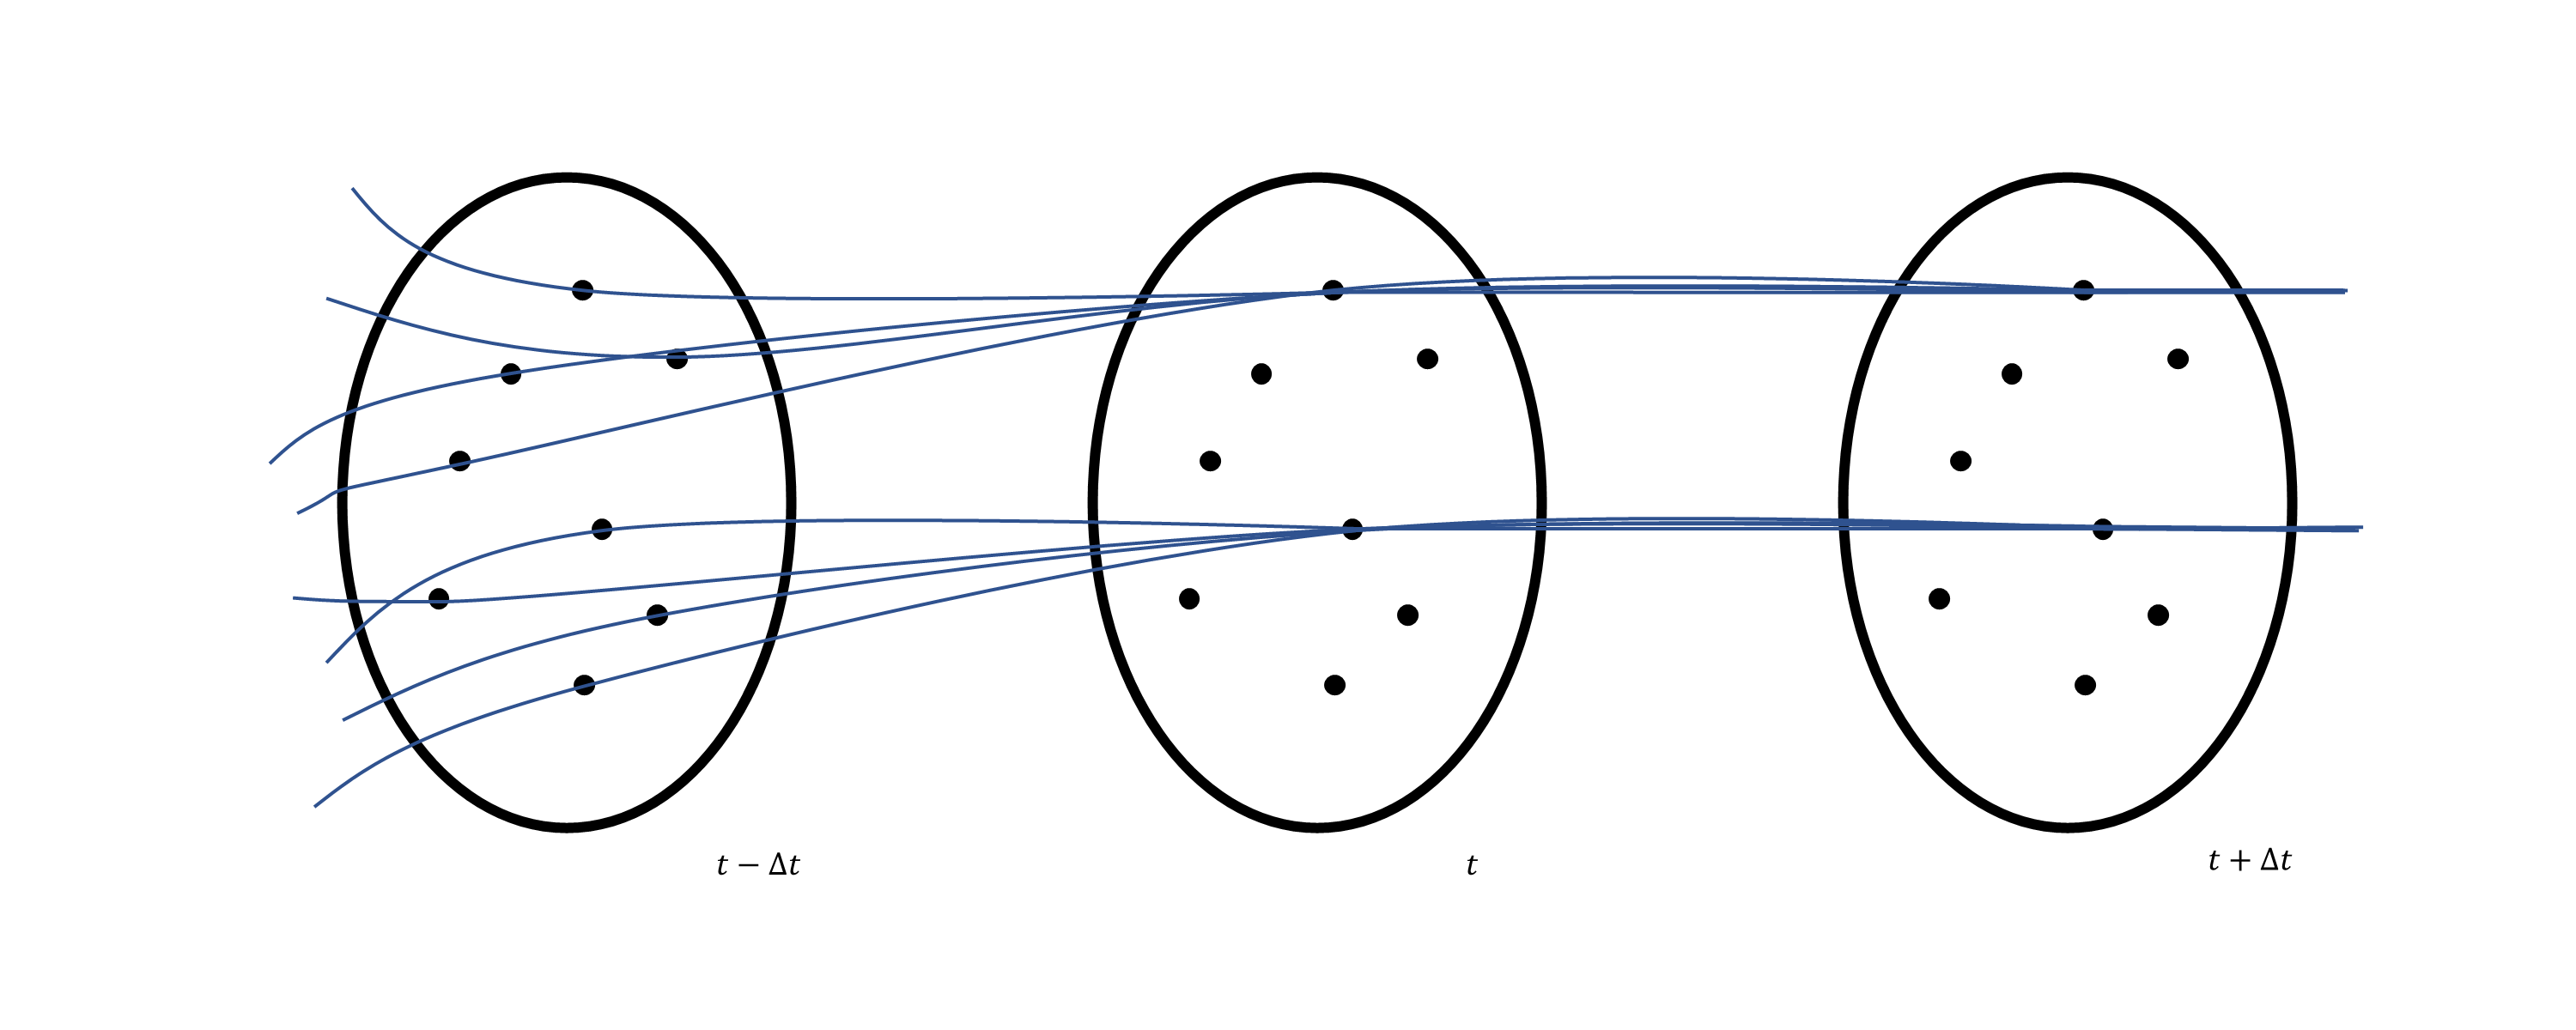
\includegraphics[width=\columnwidth]{images/Slide6.png}
	\caption{Deterministic process with equilibria. Evolutions keep merging until equilibrium is reached. The number of evolutions per state increases and the maximum is reached at equilibria.}\label{fig_with_equilibria}
\end{figure}

We already reached an important result: with only a handful of simple definitions we have found a quantity, $\mu(\lambda(t))$, that can never decrease in a deterministic process, stays the same if the process is also reversible and is maximized at equilibrium. We have done so with no assumption on the type of system, the type of forces acting on the system, the internal composition of the system or the internal dynamics of the system. It knows nothing of uncertainty, disorder, information, statistical or probability distribution, phase space volumes. It only knows about evolutions and how to count them. The result is completely general and the justification is very straight forward. It is conceptually a perfect candidate for the thermodynamic entropy, though we have one questions left: how does it combine under system composition?

Suppose we have two systems, with their respective state spaces $X$ and $Y$. The state space of the composite system is the set of all possible pairs $X \times Y$. A process defined on the composite system will come with a measure $\mu_{X \times Y}$ that enables us to count evolutions $\lambda(t) = \{\lambda_x(t), \lambda_y(t)\}$ of the composite system. In general, the evolution of one system will affect the evolution of the other system. This will not happen, however, if the systems are independent. That is, as shown in \ref{fig_independence}, for each possible evolution $\lambda_x(t)$ of the first system and $\lambda_y(t)$ of the second system, there will be a possible evolution $\{\lambda_x(t), \lambda_y(t)\}$ on the composite. In other words,
\begin{equation}
	\mu_{X \times Y} = \mu_X \mu_Y
\end{equation}
the measure factorizes. We say two systems are \textbf{independent} at a given time $t$ if the evolutions per state factorizes: $\mu_{X \times Y}(\lambda(t)) = \mu_X (\lambda_x(t)) \mu_Y (\lambda_y(t))$.

\begin{figure}[h]
	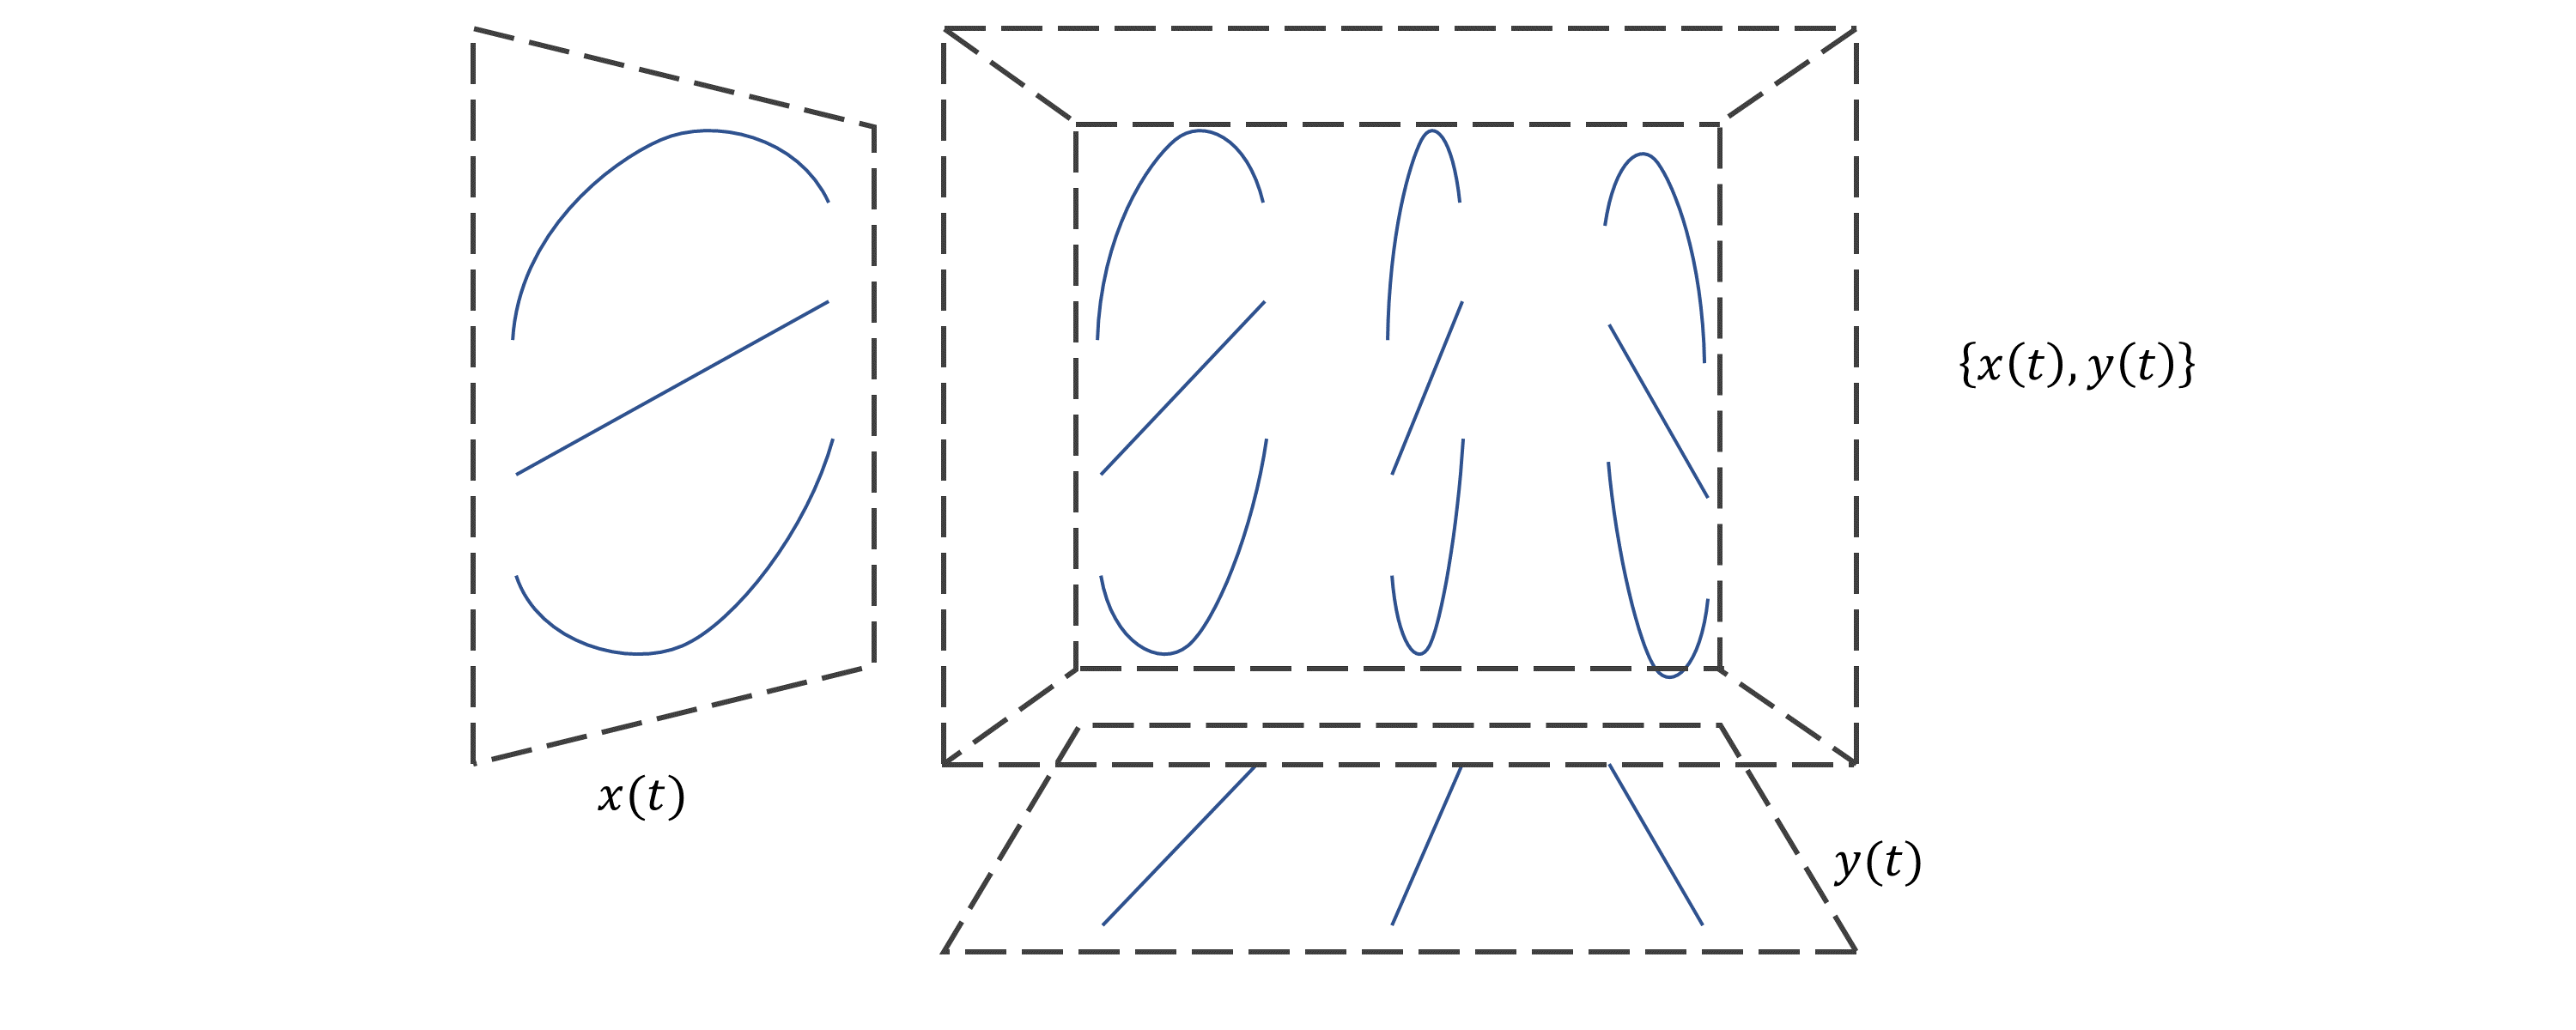
\includegraphics[width=\columnwidth]{images/Slide7.png}
	\caption{Independent system. If two systems are independent, the evolution of one does not restrict the evolution of the other: all pairs are possible. The number of evolutions factorizes.}\label{fig_independence}
\end{figure}

We define the \textbf{process entropy} as $S = \log(\mu)$. Since the logarithm is a monotonic function, the process entropy will preserve monotonicity and maximization of $\mu$ under a deterministic process with equilibria. This means:
\begin{equation}\label{ov_entropy_increases}
S(x(t)) \leq S(x(t + \Delta t))
\end{equation}
In addition, the process entropy will be additive for independent systems.\footnote{As before there are a number of technical details that need to be addressed, most of all the units for $\mu$ which will influence the 0 point for $S$. We leave these details to future works.}

Under very minimal conditions, we have found a quantity that has all the right properties for entropy and that is linked with determinism and irreversibility in a plain, intuitive and physically meaningful way. There is one remaining issue: the process entropy will depend in general on the process, not just on the state. That is, the same description of the same system may be associated with more or fewer evolutions depending on the conditions. Entropy in physics, however, is associated to a state. Under what conditions can we associate a unique process entropy to a state?

A unique value for process entropy can be assigned to states of equilibrium. Suppose, in fact, that the state $x$ is an equilibrium for two different processes $A$ and $B$. Suppose that at the end of process $A$ the system is at equilibrium $x$ and we switch to process $B$. Since $x$ is also an equilibrium for $B$, every evolution of $A$ that ended in $x$ will correspond to an evolution in $B$ that ends in $x$. By symmetry, the converse is also true. Therefore the process entropy of an equilibrium does not depend on the process, only on the equilibrium state.

For composite systems there are additional considerations. Different processes may put different degrees of correlation between subsystems, therefore the same equilibria for the subsystems may correspond to different process entropy values for the composite. But if the subsystems are independent, the composite will correspond to a unique entropy value: the product.

We can therefore assign a unique process entropy to states of equilibria and to composite states of independent equilibria. Under these conditions we define the \textbf{state entropy} $S : X \to \mathbb{R}$ which corresponds to the process entropy that the system reaches at equilibrium. Note that both equilibrium and independence lead to entropy maximization, so the state entropy can be thought as the maximal process entropy for the system. In all other cases, the process entropy will be lower meaning that that description for that system in those conditions gives us more information because of possible correlations within the system or with other systems.\footnote{This recovers the intuition of entropy as ``lack of information'' and that entropy maximization represents the case where knowledge of the system is fully represented by the given constraints. However, in our case this is not a subjective matter, rather an objective description of what the process may or may not allow.}

This link between state entropy and independent equilibria opens a series of questions on the fundamental link between the two which go beyond the scope of this paper. However, we want at least give a partial answer to one: why is assigning a unique process entropy important? One answer is process combination. Suppose that we are studying a system and we change the circumstances surrounding it: it first evolves according to process $A$ and at $t_0$ it switches to process $B$. If $\lambda(t)$ is an evolution of the combined process $AB$, then for $t \leq t_0$ it must also be an evolution for $A$ and for $t \geq t_0$ it must also be an evolution for $B$. This means that at the junction state $x_{t_0} = \lambda(t_0)$ the count of evolution has to match: $\mu_{AB}(x_{t_0})=\mu_A(x_{t_0})=\mu_B(x_{t_0})$. If we want to mix and match from a set of possible processes, then the process entropy at the junction must be only a function of the state, independent of the process. As we'll see in section \ref{sec_mechanics}, these type of consideration are already embedded in the mathematical structure of the state spaces of classical mechanics, quantum mechanics, thermodynamics and statistical mechanics.

\section{Thermodynamics}\label{sec_thermodynamics}

The above discussion sets the stage for our derivation of thermodynamics. We saw how state entropy is the maximized process entropy, a quantity that can never decrease under deterministic processes. Our task now is to extend those concepts in a way that recovers thermodynamics.

We can motivate this extension by considering process composition of composite systems. The idea is that we want to describe the situation in which a composite\footnote{Mathematically, systems under composition form a Boolean algebra. The join operation $X \cupdot Y$ returns the composite; the meet operation $X \capdot Y$ returns the smallest system contained by both; the lattice ordering $X \subseteq Y$ tells us whether $X$ is a part of $Y$ and so on.} system $X \cupdot Y$ is subject to process $A$ until time $t_0$, after which each subsystem evolves independently: $X$ according to process $B$ and $Y$ according to process $C$. At $t_0$, then, we not only have to reconcile the count of evolutions for the composite, but for each subsystem as well. Therefore $X$ and $Y$ must be independent and in equilibrium at time $t_0$. In our framework, thermodynamic equilibrium handles precisely this situation. The remaining ingredient is the notion of extensive quantities, which again serves to characterize part-whole relationships.

We define a \textbf{thermodynamic process} a particular type of deterministic process with equilibria that satisfies two additional requirements:
\begin{itemize}
	\item all parts of the systems are in equilibria and are independent from each other
	\item there is a non-trivial dependence between the initial state of one part and the final state of another (i.e. there is a way to change the initial state of one part such that the final state of another is effectively changed).
\end{itemize}
The first requirement tells us that process entropy is maximized at all levels of the system. The second requirements serves to rule out the case where the systems are isolated from each other. We say a system is in \textbf{thermodynamic equilibrium} if it is part of the output of a thermodynamic process. We say two systems are in thermodynamic equilibrium with each other if they are parts of the same system in thermodynamic equilibrium.\footnote{Mathematically, the set of all systems in the same thermodynamic equilibrium is a principal ideal $X\!\! \downarrow$.}

To get a feel for the definition, let us rederive the fact that thermodynamic equilibrium is transitive, also known as the zeroth law. Suppose system $X$ is in thermodynamic equilibrium with system $Y$ and system $Y$ is in thermodynamic equilibrium with system $Z$. Then $X$ and $Y$ are parts of the output of the same thermodynamic process and so are $Y$ and $Z$. This means that $X$ and $Z$ are parts of the output of the same thermodynamic process, and therefore are in thermodynamic equilibrium.

To characterize part-whole relationships between states, we focus on particular types of systems, which we call \textbf{thermodynamic systems}, that satisfy these additional requirements: 
\begin{itemize}
	\item the state space is formed by states of equilibria
	\item states are identified by a set of extensive quantities (i.e. additive under system composition)
	\item one such quantity, called internal energy, is conserved under all thermodynamic processes.\footnote{It may be possible that some or all of these properties can be derived from the composability of thermodynamic equilibria. Nevertheless, we consider them additional assumptions for this work.
	}
\end{itemize}
We will denote $U$ as the internal energy and $x^i$ as the remaining extensive quantities.

The next step is to characterize to what extent can thermodynamic processes change the energy and the entropy of each system. Intuitively, there are two ``orthogonal'' directions for a change of energy: constant entropy and maximal entropy change. To study these components, it is useful to consider the following special thermodynamic systems.

We say a thermodynamic system $R$ is a \textbf{thermal reservoir} if the internal energy $U_R$ is the only state variable. In this case, the equation of state is simply $S_R = S_R(U_R)$ and $\Delta S_R = \int \beta_R dU_R$.\footnote{The existence of unique equilibria between reservoirs forces $S_R(U_R)$ to be strictly monotonic.} We call \textbf{heat} $Q = - \Delta U_R$ the energy lost by the reservoir during a thermodynamic process.

We say $M$ is a \textbf{mechanical system} if the state entropy is a constant for all states. For a thermodynamic system that is also mechanical, we therefore have  $S_M(U_M, x^i_M) = k_M$ for all its states. A mechanical system cannot change entropy and all states can be connected through a deterministic and reversible process. We have:
\begin{equation}
\begin{aligned}
dU_M &= k_B T_M dS + X_{Mi} dx^i_M = X_{Mi} dx^i_M.
\end{aligned}
\end{equation}
The energy of the mechanical system is effectively \emph{stored} in one of the other state variables and can be later retrieved. We call \textbf{work} the energy exchanged by a mechanical system and we note $W=\Delta U_M$ as the energy gained by the system during a thermodynamic process.\footnote{Note that $\frac{\partial S_M}{\partial U_M} = 0 = \beta = \frac{1}{k_B T_M}$ which means the thermodynamic ``temperature'' of a mechanical system is infinite. While this ``temperature'' has little to do with thermometers, the fact that we can always transform all work into heat but not vice-versa is just a specific case of being able to move energy from higher to lower temperature.}

With these definitions, we can study how changes of energy and entropy are related to each other. Consider a system composed of a generic system $X$, a thermal reservoir $R$ and a mechanical system $M$.

During a thermodynamic process, because the total energy of the system must be conserved, we have:
\begin{equation}
\begin{aligned}
&\Delta U_X + \Delta U_R + \Delta U_M = 0 \\
&\Delta U_X - Q + W = 0 \\
&\Delta U_X = Q - W.
\end{aligned}
\end{equation}
In this setting, work represents the energy exchanged at constant entropy while heat represents exchanged energy associated with entropy change. This recovers the first law of thermodynamics.

We now look at the change in entropy, which during a thermodynamic process can never decrease given that thermodynamic processes are deterministic. Keeping in mind $M$ is mechanical, we have:
\begin{equation}
\begin{aligned}
&\Delta S_X + \Delta S_R + \Delta S_M \geq 0 \\
&\Delta S_X \geq - \Delta S_R \\
&\Delta S_X \geq \int \beta_R (- dU_R) \\
&\Delta S_X \geq \int \beta_R d Q \\
&k_B \Delta S_X \geq \int \frac{d Q}{T_R}.
\end{aligned}
\end{equation}
which recovers the second law of thermodynamics. This is just a more specialized version of \eqref{ov_entropy_increases} which is valid for any deterministic process.

The third law has many equivalent formulations. [CITE] One states that the entropy of any system has a non-negative lower bound which is reached by the lowest energy state. If the ground state is non-degenerate, such as a perfect crystal, its entropy is equal to zero. With some work, we can recover this form.

Recall that state entropy is the logarithm of the count of the possible evolutions of the system at equilibrium. The lowest possible count $\mu$ of evolutions is one, which is achieved if the equilibrium can be reached only by one starting condition. In this case, $S=\log(\mu)=0$. This tells us that state entropy is non-negative and therefore is bounded from below. We now have to show that all thermodynamic systems must have a lowest energy state and that it must be a local minimum for entropy.

First of all, the existence of unique thermodynamic equilibria forces $S(U)$ to be strictly concave (i.e. negative second derivative). This means that, at least in some region, $S(U)$ must either be a decreasing or increasing function. But since $S$ cannot be negative, $S(U)$ cannot be defined on the whole domain. Therefore $U$ must be bounded at least from above or below. Consequently, the minimum for entropy is reached either at the lowest or highest energy state. Now we show that either all thermodynamic systems must have a lowest energy state or they must have a highest energy state. Suppose, in fact, we had two systems: $X$ has no maximum energy while $Y$ has no minimum energy. Since $S_X(U_X)$ is concave, it must be a monotonically increasing function of $U_X$. This means that $\beta_X$ is always positive. Conversely, $S_X(U_X)$ must be monotonically decreasing, which means $\beta_X$ is always negative. If we put the two systems in contact, the energy of $Y$ will keep decreasing and the energy of $X$ will keep increasing and no equilibrium will ever be reached. Therefore all thermodynamic systems either have a minimum or a maximum energy. At this point the difference is a sign convention, so we can assume by convention that all thermodynamic systems have a minimum energy.

To finish, we note that a perfect crystalline structure fits the case where the system has only one possible evolution, so it is a zero entropy state. If there is degeneracy, there are different ways the equilibrium can be realized and there are different evolutions that will correspond to the same equilibrium, which means the entropy will be greater than zero. This recovers the third law.

We have thus recovered the laws of thermodynamics, and we have done so only by characterizing how equilibria and state variables behave under system composition. Apart from that, we have made no assumptions on the type of system, the type of forces acting on the system, the internal composition of the system or the internal dynamics of the system. No reference to classical mechanics, quantum mechanics or statistical mechanics is needed: the theory stands on its own. This fits the original spirit of thermodynamics, which was to find a set of laws that would be independent fn the ultimate dynamics of the constituents. This also explains the success of these ideas in fields outside physics. Additionally, the concepts we used are directly related to the physical explanation, and the laws are recovered immediately, not after pages and pages of calculations. The combination of these features makes this approach directly useful, for example, in an introductory  course: a coherent self-contained explanation can be given in terms of simple definitions.

\section{Connections to mechanics}\label{sec_mechanics}

We now want to return to the link between evolution count, state entropy and state spaces. In particular, we want to show how this link exists not only in thermodynamics, but also in classical mechanics, quantum mechanics and statistical mechanics. This is important not only to show how process entropy relates to the two main ways to define entropy in statistical mechanics, but to give a sense that all geometrical and probabilistic structure assigned to state spaces are ultimately capturing evolution counts in one way or another. This is important for our bigger project, Assumptions of Physics, as we want to create a common framework for all physical theories.

We previously defined mechanical systems as those for which all states have the same entropy. While one does not usually discuss the entropy of single classical or quantum states, it is easy to see that that must be the case. In quantum mechanics, for example, the von Neumann entropy of every pure state is zero. In classical mechanics, a uniform measure is used to count states, which means all states must contribute the same entropy. Additionally, in both theories, given two states, we can always (at least mathematically) find a deterministic and reversible process (Hamiltonian evolution and unitary evolution are entropy preserving) that starts with the first and ends in the second. So the idea that mechanical systems are associated with a constant entropy, though seldom explicit, is already embedded in the established theories.

The geometrical structure of classical mechanics, the symplectic structure of phase space, can be understood to be exactly the structure we need to count evolutions when the evolution is deterministic and reversible and the degrees of freedom are independent. In that case state entropy and process entropy coincide, but not in general. In dissipative processes, like a damped harmonic oscillator, this relationship breaks down. As the system loses energy, the evolutions gradually concentrate around the attractors. In terms of count of states, areas shrink over time, so counting states gives us a decreasing number, which is at odds with the idea of entropy increasing when progressing towards an equilibrium. What happens is that as the system evolves, each region will correspond to the same number of evolutions, which will now be spread over fewer states: the process entropy (i.e. the logarithm of the evolutions per state) increases as evolutions become more concentrated.

The mathematical structure of quantum mechanics also can be understood in terms of evolution counts. The inner product of quantum mechanics gives us the conditional probabilities of a ``black box'' process (i.e. the projection/measurements) that, given an initial state, gives us a final one. As we saw, conditional probabilities are ratios of evolution counts: what fractions of the evolutions that start in one state end in another. In other words, the inner product tells us how the evolutions coming in and coming out of these processes are to be ``joined'' with the preceding and following ones.  Moreover, note that these processes are projections, meaning they give the same result if applied more than once. Eigenstates of projections, then, are equilibria of the process the projection represents. Or, in other words, equilibria are symmetries of the process.

In statistical mechanics, one uses the above structures to define the entropy of an ensemble. There are currently two ways to do this. The first, commonly referred to as the fundamental postulate of statistical mechanics, is to take the logarithm of the state count of the region of phase space identified by the constraints (e.g. the energy of the system is within a particular bound). We can relate this to the process entropy in the following way. Suppose that the constraints are such that each microstate either is compatible or incompatible with the macrostate. Then the count of evolutions of the macrostate is the sum of all the evolutions of its microstates. Now suppose that, when the constraints are defined, the system is at equilibrium and independent. Then the process entropy is equal to the state entropy. Since the system is mechanical, the state entropy is the same for all states. This means that, if the conditions above are met, the process entropy is, up to a constant, the logarithm of the state count.\footnote{If the system starts independent and at equilibrium, for example, the entropy of a final equilibrium would correspond to the logarithm of the size of the basin of attraction: each state corresponds to a single evolution that ends in the attractor.}

The second way to define entropy is through the Gibbs and von Neumann entropies, which essentially are the application of the Shannon entropy in the classical and quantum case. This can be related to the process entropy in the following way. Suppose we have a macroscopic equilibrium which can be understood as a dynamical equilibrium of the microscopic description. That is, the macroscopic equilibrium is a set of evolutions whose microscopic description can be characterized by a stable probability distribution $\rho(x)$. An evolution $\lambda(t)$ for the microstate, then, is an dense sequence of infinitely many microstates whose recurrence matches $\rho(x)$. Since the state entropy is the maximal process entropy, we are counting all possible evolutions which means all possible permutations. The Shannon entropy can be understood as the count of all possible permutations of an infinite sequence, of all possible evolutions.

The above insights show that the framework we are setting up is not just a nicer retelling of thermodynamics, but it is something more fundamental that underlies all physical theories. Most, if not all, experiments are described as a sequence of different steps (e.g. one or more preparation, manipulation and measurement) stitched together. Making sure that the evolution count matches at every junction is a very simple and necessary bookkeeping requirement, and therefore it makes sense it plays such a major role in defining state spaces.


Therefore it makes sense that countMaking sure that the evolution count  Stitching together those phases into a single process 

The idea of using states as junctures when processes change is at the core of scientific experimentation since most experiments are 


 maostate preparation)can help us better understand the fundamental connection between all these theories. We stress that we are not arguing that all other notions of entropy should be abandoned in favor of process entropy: quite the contrary. Specific tools are often more useful than general tools precisely because they take advantage of the specific nature of the problem. The point is that if we are more aware of the interplay between the general definition and the more specific one we will not use the latter inappropriately.

\section{Conclusion and further work}

In this paper we gave a conceptual overview for a new approach to recover thermodynamics based on the simple idea of counting evolutions, the possible ways a system can evolve under a process. We saw that the logarithm of evolution count under a deterministic process has all the properties we associate with entropy. We have seen that the evolution count is maximized at equilibrium and for independent system and only in those cases it depends only on the state. A well defined evolution count is necessary if we want to be able to compose processes, since the incoming evolutions needs to match the outgoing evolutions for all states at the junction. Thermodynamics studies exactly the case of composite processes of composite systems under some simplifying conditions. This gives a simple way to rederive thermodynamics in a straight-forward and conceptually insightful way.

Moreover, we have seen that the state spaces of classical, quantum and statistical mechanics include geometrical and probabilistic structures that can all be understood in terms of evolution count. Our hope and long term goal is to develop a formal theory based on these ideas that identifies a minimum set of requirements for the definition of a state space. This theory can be further refined with additional assumptions in different ways to recover the different physical theories. We believe this would help us better understand the right questions to ask in within the foundations of physics.

\bibliography{bibliography}


\end{document}